\section{Fuzzy Risk Assessment}
\begin{frame}{$\bm{\alpha}$-cuts Based Fuzzy Bayesian Approximate Inference}
    Two problems in the inference of Bayesian network:\pause
    \begin{itemize}
      \item The operation of fuzzy probabilities would come up against a problem, where the result can produce a fuzzy probability not in the interval $[0,1]$.\pause
      \item Many algorithms have been developed for Bayesian inference, such as probability propagation in trees of clusters, variable elimination algorithm, junction tree algorithm. These exact inference algorithms are NP-hard.
    \end{itemize}

    \pause
    To solve the aforementioned problems, a novel inference algorithm named \textbf{$\bm{\alpha}$-cuts Based Fuzzy Bayesian Approximate Inference} is proposed.
\end{frame}

\begin{frame}{$\bm{\alpha}$-cuts Based Fuzzy Bayesian Approximate Inference}
    \begin{overlayarea}{\textwidth}{7cm}
    Assuming that node $x$ is a node in Bayesian network $\bnt$. Its parent node set is $\pnode{\bm{x}} = \{\pnode{x}_1, \pnode{x}_2, \cdots, \pnode{x}_m\}$ and child node set is $\cnode{\bm{x}}=\{\cnode{x}_1, \cnode{x}_2, \cdots, \cnode{x}_n\}$.
    \only<1-6>{The information spreading process is shown as following figure.
    \begin{figure}
      \centering
      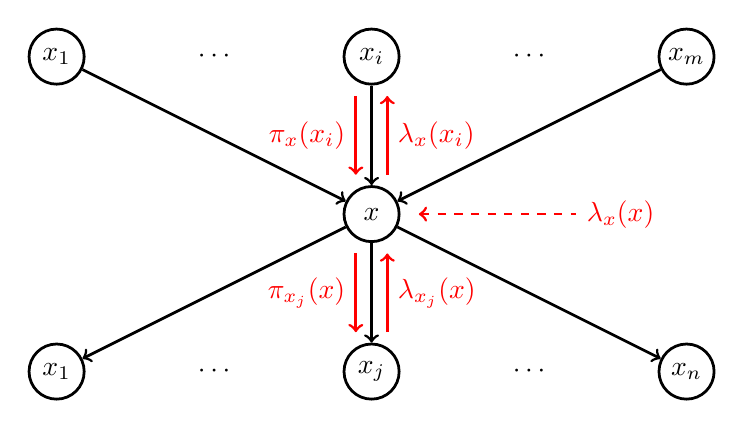
\begin{tikzpicture}[line width = 1pt,
                    node/.style = {draw, circle, inner sep = 0pt, minimum size = 0.7cm}]
    % Draw help lines.
    % \draw (0, 0) to[grid with coordinates]  (6, 8);
    
    \node[node] (cx1) at (0, 1) {$\cnode{x}_1$};
    \node             at (2, 1) {$\cdots$};
    \node[node] (cxj) at (4, 1) {$\cnode{x}_j$};
    \node             at (6, 1) {$\cdots$};
    \node[node] (cxn) at (8, 1) {$\cnode{x}_n$};

    \node[node] (px1) at (0, 5) {$\pnode{x}_1$};
    \node             at (2, 5) {$\cdots$};
    \node[node] (pxi) at (4, 5) {$\pnode{x}_i$};
    \node             at (6, 5) {$\cdots$};
    \node[node] (pxm) at (8, 5) {$\pnode{x}_m$};

    \node[node]   (x) at (4, 3) {$x$};
        
    \draw[->] (px1) -- (x);
    \draw[->] (pxi) -- (x);
    \draw[->] (pxm) -- (x);
    \draw[->] (x) -- (cx1);
    \draw[->] (x) -- (cxj);
    \draw[->] (x) -- (cxn);
    \pause

    \draw[->, red] (3.8, 4.5) -- (3.8, 3.5) node[anchor = east, midway, red] {$\pi_x(\pnode{x}_i)$};
    \pause

    \draw[->, red] (3.8, 2.5) -- (3.8, 1.5) node[anchor = east, midway, red] {$\pi_{\cnode{x}_j}(x)$};
    \pause
    
    \draw[->, red] (4.2, 1.5) -- (4.2, 2.5) node[anchor = west, midway, red] {$\lambda_{\cnode{x}_j}(x)$};
    \pause
    
    \draw[->, red] (4.2, 3.5) -- (4.2, 4.5) node[anchor = west, midway, red] {$\lambda_x(\pnode{x}_i)$};
    \pause    
    
    \draw[<-, dashed, red] (4.6, 3) -- ++(0:2cm) node[anchor = west, red] {$\lambda_x(x)$};
\end{tikzpicture}

    \end{figure}
    }
    \only<7->{At the $(t+1)\text{th}$ iteration, the message that $x$ passes to its parent node $\pnode{x}_i$ is given by following equation.
    \[
    \scalebox{0.9}{$
    \begin{bmatrix}
        \lambda_x^{(t+1)}(\pnode{x}_i = F) \\[5pt]
        \lambda_x^{(t+1)}(\pnode{x}_i = T)
    \end{bmatrix}
    = \beta
    \begin{bmatrix}
        \LambdaX{F} \\[15pt]
        \LambdaX{T}
    \end{bmatrix}$}\text{,}
    \]

    where $\pnode{\bm{x}}_i = \pnode{\bm{x}}\setminus\{\pnode{x}_i\}$. And the message that $x$ sends to its child node $\cnode{x}_j$ is given by following equation.
    \[
    \scalebox{0.9}{$
    \begin{bmatrix}
        \pi_{\cnode{x}_j}^{(t+1)}{(x = F)} \\[5pt]
        \pi_{\cnode{x}_j}^{(t+1)}{(x = T)}
    \end{bmatrix}
    = \beta
    \begin{bmatrix}
        \PiX{F} \\[15pt]
        \PiX{T}
    \end{bmatrix}$}\text{.}
    \]}
    \end{overlayarea}
\end{frame}

\begin{frame}{$\bm{\alpha}$-cuts Based Fuzzy Bayesian Approximate Inference}
    The function $\lambda_{x}(\var)$ is the message that the node $x$ sends to itself, which is presented as following equations.
    \begin{align*}
      \lambda_{x}{(x = F)} &=
        \left\{\begin{array}{ll}
        0, & \text{when $x \in \bm{E}$, and the value of observed $x$ \text is $T$,}\\[3pt]
        1, & \text{otherwise.}
        \end{array}\right.\\[5pt]
      \lambda_{x}{(x = T)} &=
        \left\{\begin{array}{ll}
        0, & \text{when $x \in \bm{E}$, and the value of observed $x$ \text is $F$,}\\[3pt]
        1, & \text{otherwise.}
        \end{array}\right.
    \end{align*}
\end{frame}

\begin{frame}{$\bm{\alpha}$-cuts Based Fuzzy Bayesian Approximate Inference}
    At the end of $(t)$th iteration, the fuzzy belief of node $x$ is given by following equation.
    \[
    \begin{bmatrix}
        {\rm Bel}^{(t)}(x = F)\\[5pt]
        {\rm Bel}^{(t)}(x = T)
    \end{bmatrix} = \beta
    \begin{bmatrix}
        \lambda^{(t)}(x = F)\cdot\pi^{(t)}(x = F)\\[5pt]
        \lambda^{(t)}(x = T)\cdot\pi^{(t)}(x = T)
    \end{bmatrix}\text{,}
    \]\pause
    where
    \begin{flalign*}
      &&
      \begin{bmatrix}
        \lambda^{(t)}(x = F)\\[5pt]
        \lambda^{(t)}(x = T)
      \end{bmatrix} & =
      \begin{bmatrix}
        \displaystyle\lambda_{x}(x = F)\prod_{j}{\lambda_{\cnode{x}_j}^{(t)}{(x = F)}} & \\[15pt]
        \displaystyle\lambda_{x}(x = T)\prod_{j}{\lambda_{\cnode{x}_j}^{(t)}{(x = T)}}
      \end{bmatrix}
      \text{,}\\
    \text{and} &&
      \begin{bmatrix}
        \pi^{(t)}(x = F) \\[5pt]
        \pi^{(t)}(x = T)
      \end{bmatrix} &=
      \begin{bmatrix}
        \displaystyle\sum_{\pnode{\bm{x}}}{P(x = F|\pnode{\bm{x}})}\prod_{k}{\pi_{x}^{(t)}{(\pnode{x}_k)}} \\[15pt]
        \displaystyle\sum_{\pnode{\bm{x}}}{P(x = T|\pnode{\bm{x}})}\prod_{k}{\pi_{x}^{(t)}{(\pnode{x}_k)}}
      \end{bmatrix}\text{.} &
    \end{flalign*}
\end{frame}

\begin{frame}{$\bm{\alpha}$-cuts Based Fuzzy Bayesian Approximate Inference}
    The iteration will be terminated when at least one of the conditions which are shown in following inequations are satisfied.
    \begin{gather*}
        t \geq t_{\max}\text{,}\\
        \forall x \in \bnt,\hspace{0.5em} D\big({\rm Bel}^{(t)}{(x = T)},{\rm Bel}^{(t-1)}{(x = T)}\big) \leq \lthreshold\text{,}
    \end{gather*}\pause
    where $D\big({\rm Bel}^{(t)}{(x = T)},{\rm Bel}^{(t-1)}{(x = T)}\big)$ represents the Hamming distance between two fuzzy numbers ${\rm Bel}^{(t)}{(x = T)}$ and ${\rm Bel}^{(t-1)}{(x = T)}$. The Hamming distance is defined as following equation.
    \[
        D\big({\rm Bel}^{(t)}{(x = T)},{\rm Bel}^{(t-1)}{(x = T)}\big)=\int _{0}^{1}{\big|\mu^{(t)}{(\rho)}-\mu^{(t-1)}{(\rho)}\big|}\dif \rho \text{.}
    \]\pause
    When the iteration is terminated, the ${\rm Bel}^{(t)}{(x)}$ is considered to be the approximate posterior fuzzy probability of node $x$ under the evidence set $\bm{E}$.
    \[
        \fp{p}(x = T|\bm{E}) \approx {\rm Bel}^{(t)}{(x = T)} \text{.}
    \]
\end{frame}

\begin{frame}{$\bm{\alpha}$-cuts Based Fuzzy Bayesian Approximate Inference}
    It is note that, there are only two kinds of operations of fuzzy probability in the inference of the fuzzy Bayesian network: addition and multiplication.\pause

    The fuzzy numbers are expressed by \acuts for calculation. For example, the triangular fuzzy probability $\fp{p}=\fpe{}$ is defined as following equation.
    \[
    \mu{(\rho)}=
    \left\{\begin{array}{@{\,}l@{}ll}
      & \dfrac{\rho-\pl{p}}{p - \pl{p}}, & \text{when $\pl{p} \leq \rho \leq p$,}\\[10pt]
    - & \dfrac{\rho-\pu{p}}{\pu{p} - p}, & \text{when $p < \rho \leq \pu{p}$,}\\[10pt]
      & 0,                               & \text{otherwise}.
    \end{array}\right.
    \]
\end{frame}

\begin{frame}{$\bm{\alpha}$-cuts Based Fuzzy Bayesian Approximate Inference}
    There are two expression of fuzzy probability:
    \begin{flalign*}
      && \fp{p} &= \fpe{}\text{,} & \\
      && \fp{p} &= \big[\ell(\alpha),u(\alpha)\big], \forall \alpha\in[0,1]\text{,} & \\
    \text{where} &&
      \ell(\alpha) &= \alpha(p-\pl{p})+\pl{p}\text{,} & \\
      && u(\alpha) &= \pu{p}-\alpha(\pu{p}-p)\text{.} &
    \end{flalign*}\pause

    The relationship between two kinds of expressions are shown in the following figure.
    \begin{figure}
      \centering
      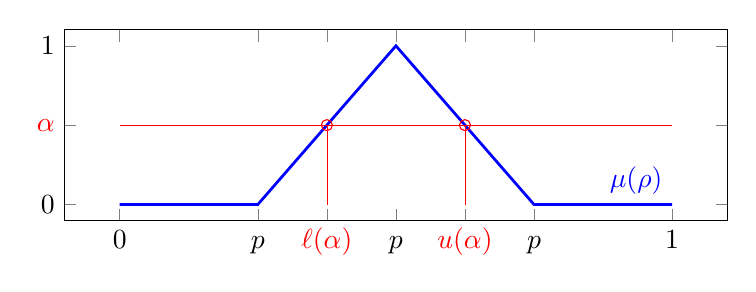
\begin{tikzpicture}
    \linespread{1}
    \begin{axis}[
        width            = 10cm,
        height           = 4cm,
        xtick            = {0, 1, 1.5, 2, 2.5, 3, 4},
        xticklabels      = {0, 
                            $\pl{p}$, 
                            \textcolor{red}{$\ell(\alpha)$}, 
                            $p$, 
                            \textcolor{red}{$u(\alpha)$}, 
                            $\pu{p}$, 
                            1},
        xticklabel style = {text height = 1.5ex},
        ytick            = {0, 0.5, 1},
        yticklabels      = {0, \textcolor{red}{$\alpha$}, 1}]

        \addplot[
            line width   = 1pt,
            mark         = none,
            draw         = blue]
            coordinates {
                (0,0)
                (1,0)
                (2,1)
                (3,0)
                (4,0)
            };
        \draw[ultra thin, red] (axis cs:0, 0.5) -- (axis cs:4, 0.5);
        \addplot[only marks, mark = o, red] coordinates {(1.5, 0.5) (2.5, 0.5)};

        \draw[ultra thin, red] (axis cs:1.5, 0.5) -- (axis cs:1.5, 0);
        \draw[ultra thin, red] (axis cs:2.5, 0.5) -- (axis cs:2.5, 0);

        \node[anchor = south east, blue] at (axis cs:4,0) {$\mu(\rho)$};
    \end{axis}
\end{tikzpicture} 
    \end{figure}
\end{frame}

\begin{frame}{$\bm{\alpha}$-cuts Based Fuzzy Bayesian Approximate Inference}
    The basic operations of addition and multiplication between fuzzy numbers used in LBP algorithm are given as following equations.
    \begin{align*}
      \action<+->{\fp{n}_1+\fp{n}_2 & = \big[\ell_1(\alpha), u_1(\alpha)\big] + \big[\ell_2(\alpha), u_2(\alpha)\big]\\
      &= \big[\ell_1(\alpha)+\ell_2(\alpha), u_1(\alpha)+u_2(\alpha)\big], \forall \alpha \in [0, 1]\text{,}\\}
      \action<+->{\fp{n}_1\times\fp{n}_2 & = \big[\ell_1(\alpha), u_1(\alpha)\big] \times \big[\ell_2(\alpha), u_2(\alpha)\big] \\
      &= \big[\ell_1(\alpha)\times\ell_2(\alpha), u_1(\alpha)\times u_2(\alpha)\big], \forall \alpha \in [0, 1]\text{.}}
      \action<+->{\intertext{It is noted that, a crisp number can be regarded as a special fuzzy number whose membership function is a unit-impulse function. Therefore, the operations between fuzzy number and crisp number are shown as following equations.}
      \fp{n}_1+n_2 &= \big[\ell_1(\alpha), u_1(\alpha)\big] + n_2 \\
      &= \big[\ell_1(\alpha)+n_2, u_1(\alpha)+n_2\big], \forall \alpha \in [0, 1]\text{,}\\}
      \action<+->{\fp{n}_1\times n_2 &= \big[\ell_1(\alpha), u_1(\alpha)\big] \times n_2 \\
      &= \big[\ell_1(\alpha)\times n_2, u_1(\alpha)\times n_2\big], \forall \alpha \in [0, 1]\text{.}}
    \end{align*}
\end{frame}

\begin{frame}{$\bm{\alpha}$-cuts Based Fuzzy Bayesian Approximate Inference}
    In this paper, the normalization algorithm developed by Dubois and Prade\footnote{ Didier Dubois and Henri Prade. The use of fuzzy numbers in decision analysis. \emph{Fuzzy information and decision processes}, pages 309–321, 1982.} are employed to normalize the fuzzy numbers. Assuming $\fp{n}_1$ and $\fp{n}_2$ are two fuzzy numbers, the normalization algorithm is shown as the following equation.
    \[
    \beta
    \begin{bmatrix}
      \fp{n}_1 \\[5pt]
      \fp{n}_2
    \end{bmatrix} =
    \begin{bmatrix}
    \bigg[\dfrac{\ell_1(\alpha)}{\ell_1(\alpha) + u_2(\alpha)}, \dfrac{u_1(\alpha)}{u_1(\alpha) + \ell_2(\alpha)}\bigg], \forall \alpha \in [0, 1]\\[15pt]
    \bigg[\dfrac{\ell_2(\alpha)}{\ell_2(\alpha) + u_1(\alpha)}, \dfrac{u_2(\alpha)}{u_2(\alpha) + \ell_1(\alpha)}\bigg], \forall \alpha \in [0, 1]
    \end{bmatrix}\text{.}
    \]
\end{frame}

\begin{frame}{$\bm{\alpha}$-cuts Based Fuzzy Bayesian Approximate Inference}
In the process of Bayesian inference, it is hard to calculate the analytical expression of the iterating results.\pause

To solve this problem that is hard to obtain the analytical expression, a compromised computation strategy is proposed. This computation strategy adopts finite interval values to represent a fuzzy number approximately.\pause

There is a set of $\alpha \in [0, 1]$ which is denoted by $\bm{\alpha} = \{\alpha_1, \alpha_2, \cdots, \alpha_n\}$, $\forall i, j = 1, 2, \cdots, n$, if $i \neq j$, then $\alpha_i \neq \alpha_j$. \pause In this paper, for a fuzzy number $\big[\ell(\alpha), u(\alpha)\big], \forall \alpha \in [0, 1]$, the proposed computation strategy is to calculate the finite interval values $\big[\ell(\alpha), u(\alpha)\big], \forall \alpha \in \bm{\alpha}$. \pause In this paper, the set of $\alpha$ which is shown in the following equation is suggested.
\[
  \bm{\alpha} = \bigg\{\alpha_i\Big| \alpha_i = \frac{i-1}{n-1}, i = 1, 2, \cdots, n\bigg\}\text{.}
\]
\end{frame}

\begin{frame}{Data Filter}
    The architecture of the data filter is shown in the following figure.

    \resizebox{\textwidth}{!}{\newkeycommand{\model}[x = 0cm, y = 0cm, width = 3.4cm, height = 1.8cm, name = model][1]{
\node[fill = white, cylinder, shape border rotate = 90, draw, minimum height = \commandkey{height}, minimum width = \commandkey{width}, align = center, shape aspect=2] (\commandkey{name}) at (\commandkey{x}, \commandkey{y}) {};

\draw[dashed, line width = 0.5pt]
let \p1 = ($ (\commandkey{name}.after bottom) - (\commandkey{name}.before bottom) $),
    \n1 = {0.5*veclen(\x1,\y1)-\pgflinewidth},
    \p2 = ($ (\commandkey{name}.bottom) - (\commandkey{name}.after bottom)!.5!(\commandkey{name}.before bottom) $),
    \n2 = {veclen(\x2,\y2)-\pgflinewidth}
in
    ([xshift=-\pgflinewidth] \commandkey{name}.before bottom) arc [start angle=0, end angle=180,
    x radius=\n1, y radius=\n2];

\coordinate (\commandkey{name}BottomCenter) at ($(\commandkey{name}.after bottom)!0.5!(\commandkey{name}.before bottom)$);
\coordinate (\commandkey{name}TopCenter) at ($(\commandkey{name}.after top)!0.5!(\commandkey{name}.before top)$);

\node at (\commandkey{x}, \commandkey{y}) [fill = white, align = center, inner sep = 1pt] {#1};
}

\newkeycommand{\lefttag}[x = 0cm, y = 0cm, width = 3cm][1]{
\node at (\commandkey{x} + 4pt, \commandkey{y}) [text shadow={[align=left, inner sep = 0pt, font = \small, anchor = west] at (\commandkey{x} + 4pt, \commandkey{y}) {\parbox{\commandkey{width}}{#1}}}, align = left, inner sep = 0pt, font = \small, anchor = west] {\parbox{\commandkey{width}}{#1}};
}

\begin{tikzpicture}[line width = 1pt,
                    block/.style = {draw, rectangle, fill =white, minimum width = 2cm, minimum height = 1.4cm, inner sep = 0pt, align = center},
                    cup/.style = {fill = black, circle, inner sep = 0pt, minimum size = 0.5cm, text = white},
                    line/.style = {draw = white, line width = 3pt}]

% \draw (0, 0) to[grid with coordinates]  (14, 9);
\linespread{1}

\fill[rounded corners, black!30] (3.8, 3.1) rectangle (11.7, 8.9);
\shadowtext[align = center] at (10.1, 7.7) {\Large \bf Data\\[5pt] \Large \bf Filter};
\pause

\node[block] (AI) at (5, 8) {Attack\\Evidences\\Pool};
\node[block] (FI) at (5, 6) {Invalidation\\Evidence\\Identifier};
\node[block] (II) at (5, 4) {Incident\\Evidence\\Identifier};
\pause

\uncover<3>{
\draw[<-] (AI) -- ++ (180:5cm);
\draw[<-] (FI) -- ++ (180:5cm);
\draw[<-] (II) -- ++ (180:5cm);
}
\shadowtext[align = left, anchor = west] at (0, 8) {Attack\\Evidences};
\shadowtext[align = left, anchor = west] at (0, 6) {Real-time\\Data};
\shadowtext[align = left, anchor = west] at (0, 4) {Real-time\\Data};
\pause

\node[cup] (CUP1) at (2, 6) {$\bm{+}$};
\node[cup] (CUP2) at (3, 4) {$\bm{+}$};
\model[x = 2.5cm, y = 1.5cm, width = 2.5cm, name = HD]{Historical\\Database};

\draw[<-] (CUP1) -- ++(180:2cm);
\draw[<-] (CUP2) -- ++(180:3cm);
\draw[->] (CUP1) -- (FI);
\draw[->] (CUP2) -- (II);
\draw[<-] (AI) -- ++(180:5cm);
\draw[line] (HDTopCenter -| CUP1) -- (CUP1);
\draw[line] (HDTopCenter -| CUP2) -- (CUP2);
\draw[->] (HDTopCenter -| CUP1) -- (CUP1);
\draw[->] (HDTopCenter -| CUP2) -- (CUP2);
\pause

\uncover<5>{
\draw[->] (AI) -- ++ (0:3.5cm);
\draw[->] (FI) -- ++ (0:3.5cm);
\draw[->] (II) -- ++ (0:3.5cm);
}
\shadowtext[align = left, anchor = west] at (6, 8) {Attack\\Evidences};
\shadowtext[align = left, anchor = west] at (6, 6) {Invalidation\\Evidences};
\shadowtext[align = left, anchor = west] at (6, 4) {Incident\\Evidences};

\pause

\node[block] (NF) at (10.5, 6) {Noise\\Filter};
\node[cup] (CUP3) at (8.5, 6) {$\bm{+}$};
\draw[->] (AI) -| (CUP3);
\draw[->] (FI) -- (CUP3);
\draw[->] (II) -| (CUP3);
\draw[->] (CUP3) -- (NF);
\pause

\model[x = 10.5cm, y = 1.5cm, width = 2cm, name = CT]{Causal\\Model};
\draw[line] (CTTopCenter) -- ++(90:0.5cm);
\draw[->] (CTTopCenter) -- (NF);
\pause

\draw[->] (NF) -- ++(0:3cm);
\shadowtext[align = center] at (12.6, 6) {Evidence\\Set $\bm{E}$};
\end{tikzpicture} }
\end{frame}

\begin{frame}{Data Filter}
    In this paper, for the invalidation evidences and the incident evidences, an index $C(x = T)$ is proposed to measure the confidence level of an evidence $x = T$, which is shown as the following equation.
    \[
      C(x = T) = \max_{\bm{p}\in\bm{P}}\Big\{
        \sum_{i=m}^n \binom{i}{n} \eta^i(1-\eta)^{n-i}
      \Big\}\text{,}
    \]\pause
    where $\bm{P}$ is the path set of node $x$, $n$ is the number of elements in path $\bm{p}$, $m$ is the number of elements in the set $\bm{p}\setminus\bm{E}$, $\eta$ is the false negatives rate of IDS. \pause If the condition which is shown in the following equation is satisfied, the evidence $x = T$ is regarded as noise evidence caused by system faults.
    \[
        C(x = T) < C_{\min}\text{,}
    \]\pause
    where $C_{\min}$ is the minimum value of evidence confidence level, and $C_{\min}$ can be equal to $2.5\%$, $5\%$, etc.
\end{frame}

\begin{frame}{Data Filter}
    If a function node $f$ has only one path $\bm{p} = \{a_1, a_2, \cdots, a_{10}\}$. Now, there are only $a_1$, $a_2$, and $a_3$ are detected by IDS, and the invalidation of this function is detected by invalidation evidence identifier. The false negatives rate of IDS $\eta = 2.5\%$ and the minimum evidence confidence level $C_{\min} = 1\%$. \pause So, the false negatives number $m$ obeys the binomial distribution $B(10,0.025)$. \pause The confidence level of evidence $f = T$ is shown as the following equation.
    \begin{align*}
        C(f = T) &= \sum_{i=7}^{10} \binom{i}{10} 0.025^i(1-0.025)^{10-i}\\
                 & = 6.8542 \cdot 10^{-10}\text{.}
    \end{align*}\pause
    Because $C(f = T) = 6.8542 \cdot 10^{-10} < C_{\min}$, the evidence $f = T$ is a noise evidence.
\end{frame}

\begin{frame}{Risk Assessment}
    The evidences generated by attack evidence pool, invalidation evidence identifier, and incident evidence identifier, are sent to the noise filter. \pause The \abfbai{} engine receives the evidences without noise caused by system faults, then calculates the fuzzy probabilities of all asset nodes $\fp{p}(z)$. \pause At last, the current cybersecurity risk can be assessed by the following equation.
    \[
    \fp{\risk}=\sum_{z\in\bnt}{\fp{p}{(z)}\cdot v(z)}\text{,}
    \]\pause
    where $v(z)$ is the value of the asset $z$.
\end{frame}
